\documentclass[11pt]{book}

\usepackage{figureflt}
\usepackage{pgf}
\usepackage{tikz}
\usepackage{pgflibraryshapes}

\begin{document}
\date{today}


%% Plot generated by GroupOutput of alignapi
\begin{floatingigure}[r]{6.5cm}
\begin{figure}[!h]
\begin{center}
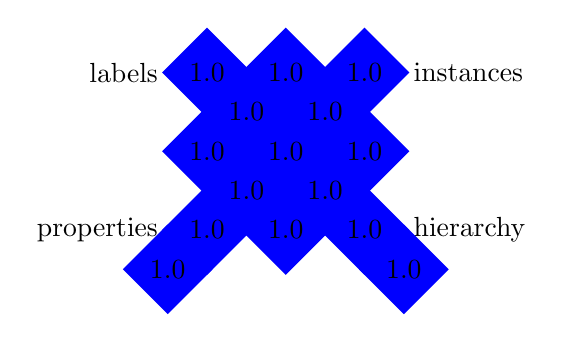
\begin{tikzpicture}
\draw (-.5,2.) node[anchor=east] {labels};
\draw (0,2.) node[diamond,minimum size=.5cm,fill=blue!100] {1.0}; % l
\draw (0,1.) node[diamond,minimum size=.5cm,fill=blue!100] {1.0}; % lp
\draw (0.5,1.5) node[diamond,minimum size=.5cm,fill=blue!100] {1.0}; % lip
\draw (1.,2.) node[diamond,minimum size=.5cm,fill=blue!100] {1.0}; %li

\draw (-.5,0.) node[anchor=east] {properties};
\draw (-0.5,-0.5) node[diamond,minimum size=.5cm,fill=blue!100] {1.0}; % ip
\draw (0,0) node[diamond,minimum size=.5cm,fill=blue!100] {1.0}; %p
\draw (.5,.5) node[diamond,minimum size=.5cm,fill=blue!100] {1.0}; % lph
\draw (1.,1.) node[diamond,minimum size=.5cm,fill=blue!100] {1.0}; % liph
\draw (1.5,1.5) node[diamond,minimum size=.5cm,fill=blue!100] {1.0}; %hil
\draw (2.,2.) node[diamond,minimum size=.5cm,fill=blue!100] {1.0}; %i
\draw (2.5,2.0) node[anchor=west] {instances};

\draw (2.,1.) node[diamond,minimum size=.5cm,fill=blue!100] {1.0}; % hi
\draw (1.5,0.5) node[diamond,minimum size=.5cm,fill=blue!100] {1.0}; % phi
\draw (1.,0) node[diamond,minimum size=.5cm,fill=blue!100] {1.0}; % ph
\draw (2.,0) node[diamond,minimum size=.5cm,fill=blue!100] {1.0}; % h
\draw (2.5,0.) node[anchor=west] {hierarchy};
\draw (2.5,-0.5) node[diamond,minimum size=.5cm,fill=blue!100] {1.0}; % hl
\end{tikzpicture} 
\caption{refalign evaluation on F-measure (the darkest the best).}\label{fig:diagrefalign}
\end{center}
\end{floatingfigure}

%% Plot generated by GroupOutput of alignapi
\begin{floatingigure}[r]{6.5cm}
\begin{figure}[!h]
\begin{center}
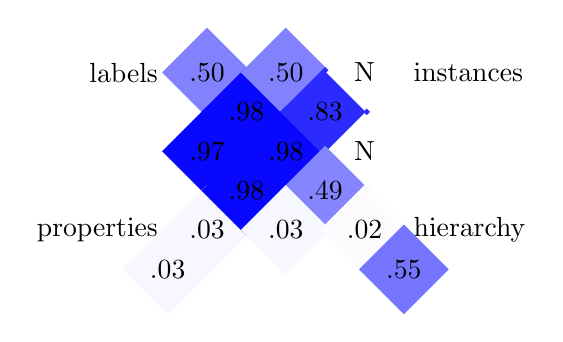
\begin{tikzpicture}
\draw (-.5,2.) node[anchor=east] {labels};
\draw (0,2.) node[diamond,minimum size=.5cm,fill=blue!49] {.50}; % l
\draw (0,1.) node[diamond,minimum size=.5cm,fill=blue!97] {.97}; % lp
\draw (0.5,1.5) node[diamond,minimum size=.5cm,fill=blue!97] {.98}; % lip
\draw (1.,2.) node[diamond,minimum size=.5cm,fill=blue!49] {.50}; %li

\draw (-.5,0.) node[anchor=east] {properties};
\draw (-0.5,-0.5) node[diamond,minimum size=.5cm,fill=blue!3] {.03}; % ip
\draw (0,0) node[diamond,minimum size=.5cm,fill=blue!3] {.03}; %p
\draw (.5,.5) node[diamond,minimum size=.5cm,fill=blue!97] {.98}; % lph
\draw (1.,1.) node[diamond,minimum size=.5cm,fill=blue!97] {.98}; % liph
\draw (1.5,1.5) node[diamond,minimum size=.5cm,fill=blue!83] {.83}; %hil
\draw (2.,2.) node[diamond,minimum size=.5cm,fill=blue!0] {N}; %i
\draw (2.5,2.0) node[anchor=west] {instances};

\draw (2.,1.) node[diamond,minimum size=.5cm,fill=blue!0] {N}; % hi
\draw (1.5,0.5) node[diamond,minimum size=.5cm,fill=blue!48] {.49}; % phi
\draw (1.,0) node[diamond,minimum size=.5cm,fill=blue!3] {.03}; % ph
\draw (2.,0) node[diamond,minimum size=.5cm,fill=blue!1] {.02}; % h
\draw (2.5,0.) node[anchor=west] {hierarchy};
\draw (2.5,-0.5) node[diamond,minimum size=.5cm,fill=blue!54] {.55}; % hl
\end{tikzpicture} 
\caption{edna evaluation on F-measure (the darkest the best).}\label{fig:diagedna}
\end{center}
\end{floatingfigure}

%% Plot generated by GroupOutput of alignapi
\begin{floatingigure}[r]{6.5cm}
\begin{figure}[!h]
\begin{center}
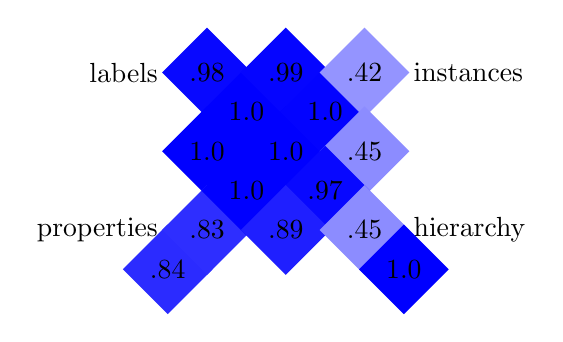
\begin{tikzpicture}
\draw (-.5,2.) node[anchor=east] {labels};
\draw (0,2.) node[diamond,minimum size=.5cm,fill=blue!97] {.98}; % l
\draw (0,1.) node[diamond,minimum size=.5cm,fill=blue!100] {1.0}; % lp
\draw (0.5,1.5) node[diamond,minimum size=.5cm,fill=blue!100] {1.0}; % lip
\draw (1.,2.) node[diamond,minimum size=.5cm,fill=blue!98] {.99}; %li

\draw (-.5,0.) node[anchor=east] {properties};
\draw (-0.5,-0.5) node[diamond,minimum size=.5cm,fill=blue!83] {.84}; % ip
\draw (0,0) node[diamond,minimum size=.5cm,fill=blue!82] {.83}; %p
\draw (.5,.5) node[diamond,minimum size=.5cm,fill=blue!100] {1.0}; % lph
\draw (1.,1.) node[diamond,minimum size=.5cm,fill=blue!100] {1.0}; % liph
\draw (1.5,1.5) node[diamond,minimum size=.5cm,fill=blue!99] {1.0}; %hil
\draw (2.,2.) node[diamond,minimum size=.5cm,fill=blue!42] {.42}; %i
\draw (2.5,2.0) node[anchor=west] {instances};

\draw (2.,1.) node[diamond,minimum size=.5cm,fill=blue!45] {.45}; % hi
\draw (1.5,0.5) node[diamond,minimum size=.5cm,fill=blue!97] {.97}; % phi
\draw (1.,0) node[diamond,minimum size=.5cm,fill=blue!88] {.89}; % ph
\draw (2.,0) node[diamond,minimum size=.5cm,fill=blue!45] {.45}; % h
\draw (2.5,0.) node[anchor=west] {hierarchy};
\draw (2.5,-0.5) node[diamond,minimum size=.5cm,fill=blue!100] {1.0}; % hl
\end{tikzpicture} 
\caption{ASMOV evaluation on F-measure (the darkest the best).}\label{fig:diagASMOV}
\end{center}
\end{floatingfigure}

%% Plot generated by GroupOutput of alignapi
\begin{floatingigure}[r]{6.5cm}
\begin{figure}[!h]
\begin{center}
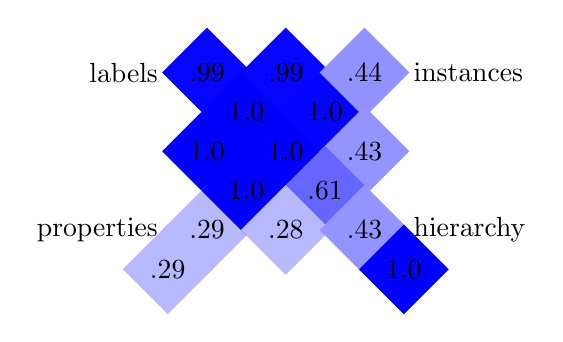
\begin{tikzpicture}
\draw (-.5,2.) node[anchor=east] {labels};
\draw (0,2.) node[diamond,minimum size=.5cm,fill=blue!98] {.99}; % l
\draw (0,1.) node[diamond,minimum size=.5cm,fill=blue!100] {1.0}; % lp
\draw (0.5,1.5) node[diamond,minimum size=.5cm,fill=blue!100] {1.0}; % lip
\draw (1.,2.) node[diamond,minimum size=.5cm,fill=blue!98] {.99}; %li

\draw (-.5,0.) node[anchor=east] {properties};
\draw (-0.5,-0.5) node[diamond,minimum size=.5cm,fill=blue!28] {.29}; % ip
\draw (0,0) node[diamond,minimum size=.5cm,fill=blue!28] {.29}; %p
\draw (.5,.5) node[diamond,minimum size=.5cm,fill=blue!100] {1.0}; % lph
\draw (1.,1.) node[diamond,minimum size=.5cm,fill=blue!100] {1.0}; % liph
\draw (1.5,1.5) node[diamond,minimum size=.5cm,fill=blue!99] {1.0}; %hil
\draw (2.,2.) node[diamond,minimum size=.5cm,fill=blue!43] {.44}; %i
\draw (2.5,2.0) node[anchor=west] {instances};

\draw (2.,1.) node[diamond,minimum size=.5cm,fill=blue!42] {.43}; % hi
\draw (1.5,0.5) node[diamond,minimum size=.5cm,fill=blue!60] {.61}; % phi
\draw (1.,0) node[diamond,minimum size=.5cm,fill=blue!28] {.28}; % ph
\draw (2.,0) node[diamond,minimum size=.5cm,fill=blue!42] {.43}; % h
\draw (2.5,0.) node[anchor=west] {hierarchy};
\draw (2.5,-0.5) node[diamond,minimum size=.5cm,fill=blue!100] {1.0}; % hl
\end{tikzpicture} 
\caption{DSSim evaluation on F-measure (the darkest the best).}\label{fig:diagDSSim}
\end{center}
\end{floatingfigure}

%% Plot generated by GroupOutput of alignapi
\begin{floatingigure}[r]{6.5cm}
\begin{figure}[!h]
\begin{center}
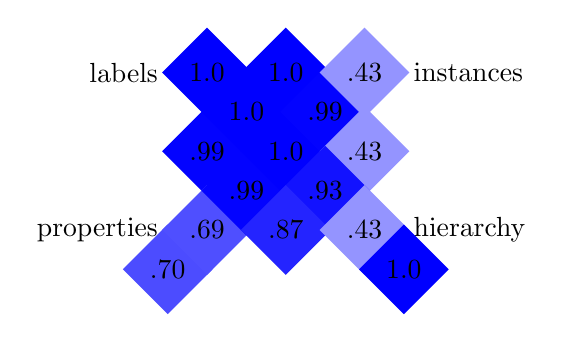
\begin{tikzpicture}
\draw (-.5,2.) node[anchor=east] {labels};
\draw (0,2.) node[diamond,minimum size=.5cm,fill=blue!100] {1.0}; % l
\draw (0,1.) node[diamond,minimum size=.5cm,fill=blue!99] {.99}; % lp
\draw (0.5,1.5) node[diamond,minimum size=.5cm,fill=blue!100] {1.0}; % lip
\draw (1.,2.) node[diamond,minimum size=.5cm,fill=blue!100] {1.0}; %li

\draw (-.5,0.) node[anchor=east] {properties};
\draw (-0.5,-0.5) node[diamond,minimum size=.5cm,fill=blue!70] {.70}; % ip
\draw (0,0) node[diamond,minimum size=.5cm,fill=blue!69] {.69}; %p
\draw (.5,.5) node[diamond,minimum size=.5cm,fill=blue!99] {.99}; % lph
\draw (1.,1.) node[diamond,minimum size=.5cm,fill=blue!100] {1.0}; % liph
\draw (1.5,1.5) node[diamond,minimum size=.5cm,fill=blue!99] {.99}; %hil
\draw (2.,2.) node[diamond,minimum size=.5cm,fill=blue!42] {.43}; %i
\draw (2.5,2.0) node[anchor=west] {instances};

\draw (2.,1.) node[diamond,minimum size=.5cm,fill=blue!42] {.43}; % hi
\draw (1.5,0.5) node[diamond,minimum size=.5cm,fill=blue!93] {.93}; % phi
\draw (1.,0) node[diamond,minimum size=.5cm,fill=blue!86] {.87}; % ph
\draw (2.,0) node[diamond,minimum size=.5cm,fill=blue!42] {.43}; % h
\draw (2.5,0.) node[anchor=west] {hierarchy};
\draw (2.5,-0.5) node[diamond,minimum size=.5cm,fill=blue!100] {1.0}; % hl
\end{tikzpicture} 
\caption{falcon evaluation on F-measure (the darkest the best).}\label{fig:diagfalcon}
\end{center}
\end{floatingfigure}

%% Plot generated by GroupOutput of alignapi
\begin{floatingigure}[r]{6.5cm}
\begin{figure}[!h]
\begin{center}
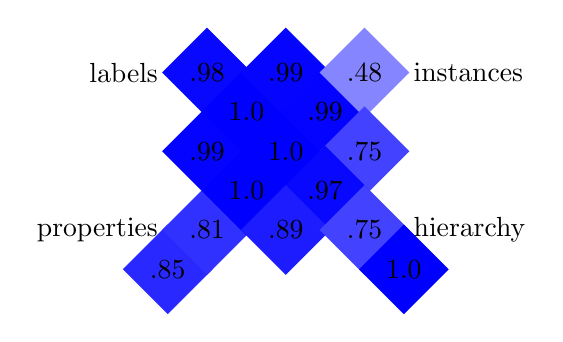
\begin{tikzpicture}
\draw (-.5,2.) node[anchor=east] {labels};
\draw (0,2.) node[diamond,minimum size=.5cm,fill=blue!97] {.98}; % l
\draw (0,1.) node[diamond,minimum size=.5cm,fill=blue!99] {.99}; % lp
\draw (0.5,1.5) node[diamond,minimum size=.5cm,fill=blue!100] {1.0}; % lip
\draw (1.,2.) node[diamond,minimum size=.5cm,fill=blue!98] {.99}; %li

\draw (-.5,0.) node[anchor=east] {properties};
\draw (-0.5,-0.5) node[diamond,minimum size=.5cm,fill=blue!84] {.85}; % ip
\draw (0,0) node[diamond,minimum size=.5cm,fill=blue!81] {.81}; %p
\draw (.5,.5) node[diamond,minimum size=.5cm,fill=blue!100] {1.0}; % lph
\draw (1.,1.) node[diamond,minimum size=.5cm,fill=blue!100] {1.0}; % liph
\draw (1.5,1.5) node[diamond,minimum size=.5cm,fill=blue!99] {.99}; %hil
\draw (2.,2.) node[diamond,minimum size=.5cm,fill=blue!48] {.48}; %i
\draw (2.5,2.0) node[anchor=west] {instances};

\draw (2.,1.) node[diamond,minimum size=.5cm,fill=blue!74] {.75}; % hi
\draw (1.5,0.5) node[diamond,minimum size=.5cm,fill=blue!97] {.97}; % phi
\draw (1.,0) node[diamond,minimum size=.5cm,fill=blue!89] {.89}; % ph
\draw (2.,0) node[diamond,minimum size=.5cm,fill=blue!74] {.75}; % h
\draw (2.5,0.) node[anchor=west] {hierarchy};
\draw (2.5,-0.5) node[diamond,minimum size=.5cm,fill=blue!100] {1.0}; % hl
\end{tikzpicture} 
\caption{lily evaluation on F-measure (the darkest the best).}\label{fig:diaglily}
\end{center}
\end{floatingfigure}

%% Plot generated by GroupOutput of alignapi
\begin{floatingigure}[r]{6.5cm}
\begin{figure}[!h]
\begin{center}
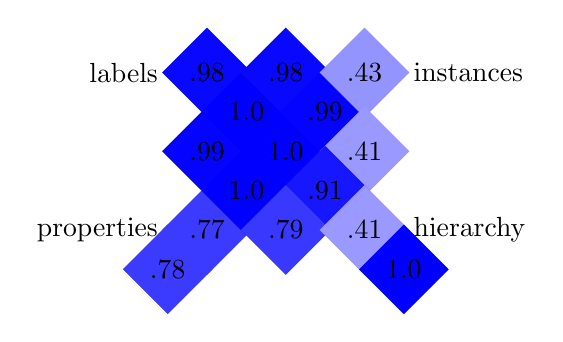
\begin{tikzpicture}
\draw (-.5,2.) node[anchor=east] {labels};
\draw (0,2.) node[diamond,minimum size=.5cm,fill=blue!97] {.98}; % l
\draw (0,1.) node[diamond,minimum size=.5cm,fill=blue!99] {.99}; % lp
\draw (0.5,1.5) node[diamond,minimum size=.5cm,fill=blue!100] {1.0}; % lip
\draw (1.,2.) node[diamond,minimum size=.5cm,fill=blue!97] {.98}; %li

\draw (-.5,0.) node[anchor=east] {properties};
\draw (-0.5,-0.5) node[diamond,minimum size=.5cm,fill=blue!77] {.78}; % ip
\draw (0,0) node[diamond,minimum size=.5cm,fill=blue!77] {.77}; %p
\draw (.5,.5) node[diamond,minimum size=.5cm,fill=blue!100] {1.0}; % lph
\draw (1.,1.) node[diamond,minimum size=.5cm,fill=blue!100] {1.0}; % liph
\draw (1.5,1.5) node[diamond,minimum size=.5cm,fill=blue!99] {.99}; %hil
\draw (2.,2.) node[diamond,minimum size=.5cm,fill=blue!42] {.43}; %i
\draw (2.5,2.0) node[anchor=west] {instances};

\draw (2.,1.) node[diamond,minimum size=.5cm,fill=blue!40] {.41}; % hi
\draw (1.5,0.5) node[diamond,minimum size=.5cm,fill=blue!91] {.91}; % phi
\draw (1.,0) node[diamond,minimum size=.5cm,fill=blue!78] {.79}; % ph
\draw (2.,0) node[diamond,minimum size=.5cm,fill=blue!40] {.41}; % h
\draw (2.5,0.) node[anchor=west] {hierarchy};
\draw (2.5,-0.5) node[diamond,minimum size=.5cm,fill=blue!100] {1.0}; % hl
\end{tikzpicture} 
\caption{ola evaluation on F-measure (the darkest the best).}\label{fig:diagola}
\end{center}
\end{floatingfigure}

%% Plot generated by GroupOutput of alignapi
\begin{floatingigure}[r]{6.5cm}
\begin{figure}[!h]
\begin{center}
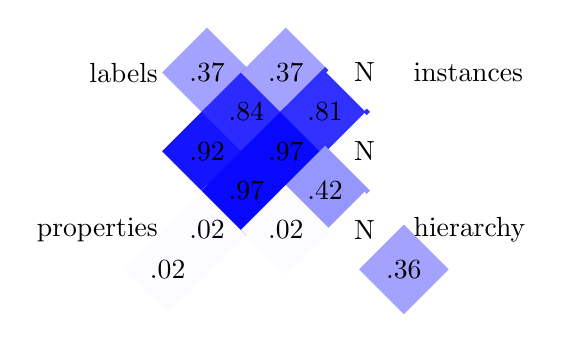
\begin{tikzpicture}
\draw (-.5,2.) node[anchor=east] {labels};
\draw (0,2.) node[diamond,minimum size=.5cm,fill=blue!36] {.37}; % l
\draw (0,1.) node[diamond,minimum size=.5cm,fill=blue!92] {.92}; % lp
\draw (0.5,1.5) node[diamond,minimum size=.5cm,fill=blue!83] {.84}; % lip
\draw (1.,2.) node[diamond,minimum size=.5cm,fill=blue!36] {.37}; %li

\draw (-.5,0.) node[anchor=east] {properties};
\draw (-0.5,-0.5) node[diamond,minimum size=.5cm,fill=blue!1] {.02}; % ip
\draw (0,0) node[diamond,minimum size=.5cm,fill=blue!1] {.02}; %p
\draw (.5,.5) node[diamond,minimum size=.5cm,fill=blue!97] {.97}; % lph
\draw (1.,1.) node[diamond,minimum size=.5cm,fill=blue!97] {.97}; % liph
\draw (1.5,1.5) node[diamond,minimum size=.5cm,fill=blue!81] {.81}; %hil
\draw (2.,2.) node[diamond,minimum size=.5cm,fill=blue!0] {N}; %i
\draw (2.5,2.0) node[anchor=west] {instances};

\draw (2.,1.) node[diamond,minimum size=.5cm,fill=blue!0] {N}; % hi
\draw (1.5,0.5) node[diamond,minimum size=.5cm,fill=blue!41] {.42}; % phi
\draw (1.,0) node[diamond,minimum size=.5cm,fill=blue!1] {.02}; % ph
\draw (2.,0) node[diamond,minimum size=.5cm,fill=blue!0] {N}; % h
\draw (2.5,0.) node[anchor=west] {hierarchy};
\draw (2.5,-0.5) node[diamond,minimum size=.5cm,fill=blue!36] {.36}; % hl
\end{tikzpicture} 
\caption{OntoDNA evaluation on F-measure (the darkest the best).}\label{fig:diagOntoDNA}
\end{center}
\end{floatingfigure}

%% Plot generated by GroupOutput of alignapi
\begin{floatingigure}[r]{6.5cm}
\begin{figure}[!h]
\begin{center}
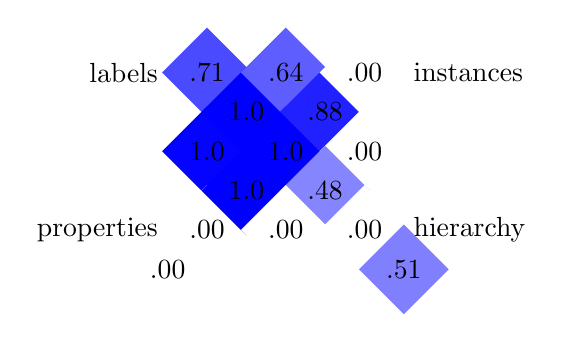
\begin{tikzpicture}
\draw (-.5,2.) node[anchor=east] {labels};
\draw (0,2.) node[diamond,minimum size=.5cm,fill=blue!71] {.71}; % l
\draw (0,1.) node[diamond,minimum size=.5cm,fill=blue!99] {1.0}; % lp
\draw (0.5,1.5) node[diamond,minimum size=.5cm,fill=blue!100] {1.0}; % lip
\draw (1.,2.) node[diamond,minimum size=.5cm,fill=blue!63] {.64}; %li

\draw (-.5,0.) node[anchor=east] {properties};
\draw (-0.5,-0.5) node[diamond,minimum size=.5cm,fill=blue!0] {.00}; % ip
\draw (0,0) node[diamond,minimum size=.5cm,fill=blue!0] {.00}; %p
\draw (.5,.5) node[diamond,minimum size=.5cm,fill=blue!100] {1.0}; % lph
\draw (1.,1.) node[diamond,minimum size=.5cm,fill=blue!100] {1.0}; % liph
\draw (1.5,1.5) node[diamond,minimum size=.5cm,fill=blue!87] {.88}; %hil
\draw (2.,2.) node[diamond,minimum size=.5cm,fill=blue!0] {.00}; %i
\draw (2.5,2.0) node[anchor=west] {instances};

\draw (2.,1.) node[diamond,minimum size=.5cm,fill=blue!0] {.00}; % hi
\draw (1.5,0.5) node[diamond,minimum size=.5cm,fill=blue!48] {.48}; % phi
\draw (1.,0) node[diamond,minimum size=.5cm,fill=blue!0] {.00}; % ph
\draw (2.,0) node[diamond,minimum size=.5cm,fill=blue!0] {.00}; % h
\draw (2.5,0.) node[anchor=west] {hierarchy};
\draw (2.5,-0.5) node[diamond,minimum size=.5cm,fill=blue!50] {.51}; % hl
\end{tikzpicture} 
\caption{OWL-CM evaluation on F-measure (the darkest the best).}\label{fig:diagOWL-CM}
\end{center}
\end{floatingfigure}

%% Plot generated by GroupOutput of alignapi
\begin{floatingigure}[r]{6.5cm}
\begin{figure}[!h]
\begin{center}
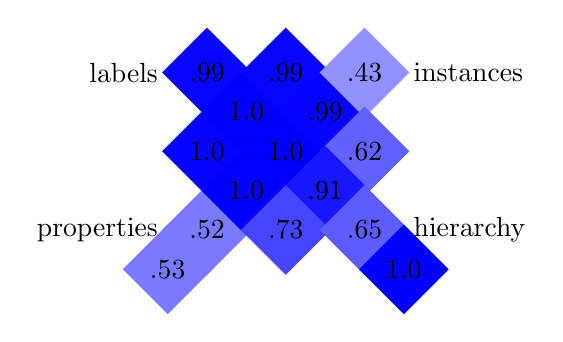
\begin{tikzpicture}
\draw (-.5,2.) node[anchor=east] {labels};
\draw (0,2.) node[diamond,minimum size=.5cm,fill=blue!98] {.99}; % l
\draw (0,1.) node[diamond,minimum size=.5cm,fill=blue!99] {1.0}; % lp
\draw (0.5,1.5) node[diamond,minimum size=.5cm,fill=blue!100] {1.0}; % lip
\draw (1.,2.) node[diamond,minimum size=.5cm,fill=blue!98] {.99}; %li

\draw (-.5,0.) node[anchor=east] {properties};
\draw (-0.5,-0.5) node[diamond,minimum size=.5cm,fill=blue!52] {.53}; % ip
\draw (0,0) node[diamond,minimum size=.5cm,fill=blue!52] {.52}; %p
\draw (.5,.5) node[diamond,minimum size=.5cm,fill=blue!100] {1.0}; % lph
\draw (1.,1.) node[diamond,minimum size=.5cm,fill=blue!100] {1.0}; % liph
\draw (1.5,1.5) node[diamond,minimum size=.5cm,fill=blue!99] {.99}; %hil
\draw (2.,2.) node[diamond,minimum size=.5cm,fill=blue!43] {.43}; %i
\draw (2.5,2.0) node[anchor=west] {instances};

\draw (2.,1.) node[diamond,minimum size=.5cm,fill=blue!62] {.62}; % hi
\draw (1.5,0.5) node[diamond,minimum size=.5cm,fill=blue!91] {.91}; % phi
\draw (1.,0) node[diamond,minimum size=.5cm,fill=blue!73] {.73}; % ph
\draw (2.,0) node[diamond,minimum size=.5cm,fill=blue!64] {.65}; % h
\draw (2.5,0.) node[anchor=west] {hierarchy};
\draw (2.5,-0.5) node[diamond,minimum size=.5cm,fill=blue!100] {1.0}; % hl
\end{tikzpicture} 
\caption{priorplus evaluation on F-measure (the darkest the best).}\label{fig:diagpriorplus}
\end{center}
\end{floatingfigure}

%% Plot generated by GroupOutput of alignapi
\begin{floatingigure}[r]{6.5cm}
\begin{figure}[!h]
\begin{center}
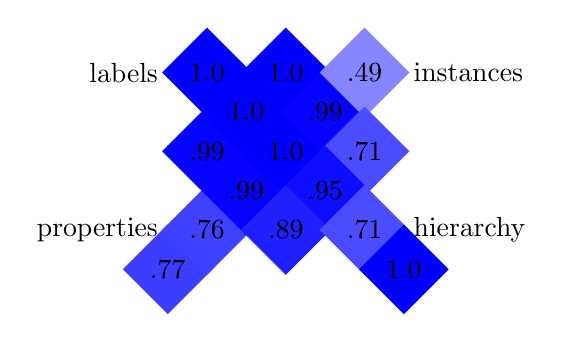
\begin{tikzpicture}
\draw (-.5,2.) node[anchor=east] {labels};
\draw (0,2.) node[diamond,minimum size=.5cm,fill=blue!100] {1.0}; % l
\draw (0,1.) node[diamond,minimum size=.5cm,fill=blue!99] {.99}; % lp
\draw (0.5,1.5) node[diamond,minimum size=.5cm,fill=blue!100] {1.0}; % lip
\draw (1.,2.) node[diamond,minimum size=.5cm,fill=blue!100] {1.0}; %li

\draw (-.5,0.) node[anchor=east] {properties};
\draw (-0.5,-0.5) node[diamond,minimum size=.5cm,fill=blue!76] {.77}; % ip
\draw (0,0) node[diamond,minimum size=.5cm,fill=blue!75] {.76}; %p
\draw (.5,.5) node[diamond,minimum size=.5cm,fill=blue!99] {.99}; % lph
\draw (1.,1.) node[diamond,minimum size=.5cm,fill=blue!100] {1.0}; % liph
\draw (1.5,1.5) node[diamond,minimum size=.5cm,fill=blue!99] {.99}; %hil
\draw (2.,2.) node[diamond,minimum size=.5cm,fill=blue!48] {.49}; %i
\draw (2.5,2.0) node[anchor=west] {instances};

\draw (2.,1.) node[diamond,minimum size=.5cm,fill=blue!70] {.71}; % hi
\draw (1.5,0.5) node[diamond,minimum size=.5cm,fill=blue!95] {.95}; % phi
\draw (1.,0) node[diamond,minimum size=.5cm,fill=blue!88] {.89}; % ph
\draw (2.,0) node[diamond,minimum size=.5cm,fill=blue!70] {.71}; % h
\draw (2.5,0.) node[anchor=west] {hierarchy};
\draw (2.5,-0.5) node[diamond,minimum size=.5cm,fill=blue!100] {1.0}; % hl
\end{tikzpicture} 
\caption{RiMOM evaluation on F-measure (the darkest the best).}\label{fig:diagRiMOM}
\end{center}
\end{floatingfigure}

%% Plot generated by GroupOutput of alignapi
\begin{floatingigure}[r]{6.5cm}
\begin{figure}[!h]
\begin{center}
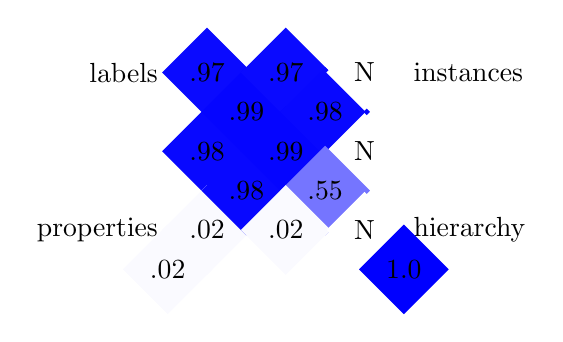
\begin{tikzpicture}
\draw (-.5,2.) node[anchor=east] {labels};
\draw (0,2.) node[diamond,minimum size=.5cm,fill=blue!96] {.97}; % l
\draw (0,1.) node[diamond,minimum size=.5cm,fill=blue!97] {.98}; % lp
\draw (0.5,1.5) node[diamond,minimum size=.5cm,fill=blue!98] {.99}; % lip
\draw (1.,2.) node[diamond,minimum size=.5cm,fill=blue!96] {.97}; %li

\draw (-.5,0.) node[anchor=east] {properties};
\draw (-0.5,-0.5) node[diamond,minimum size=.5cm,fill=blue!2] {.02}; % ip
\draw (0,0) node[diamond,minimum size=.5cm,fill=blue!2] {.02}; %p
\draw (.5,.5) node[diamond,minimum size=.5cm,fill=blue!97] {.98}; % lph
\draw (1.,1.) node[diamond,minimum size=.5cm,fill=blue!98] {.99}; % liph
\draw (1.5,1.5) node[diamond,minimum size=.5cm,fill=blue!97] {.98}; %hil
\draw (2.,2.) node[diamond,minimum size=.5cm,fill=blue!0] {N}; %i
\draw (2.5,2.0) node[anchor=west] {instances};

\draw (2.,1.) node[diamond,minimum size=.5cm,fill=blue!0] {N}; % hi
\draw (1.5,0.5) node[diamond,minimum size=.5cm,fill=blue!54] {.55}; % phi
\draw (1.,0) node[diamond,minimum size=.5cm,fill=blue!2] {.02}; % ph
\draw (2.,0) node[diamond,minimum size=.5cm,fill=blue!0] {N}; % h
\draw (2.5,0.) node[anchor=west] {hierarchy};
\draw (2.5,-0.5) node[diamond,minimum size=.5cm,fill=blue!100] {1.0}; % hl
\end{tikzpicture} 
\caption{sambo evaluation on F-measure (the darkest the best).}\label{fig:diagsambo}
\end{center}
\end{floatingfigure}

%% Plot generated by GroupOutput of alignapi
\begin{floatingigure}[r]{6.5cm}
\begin{figure}[!h]
\begin{center}
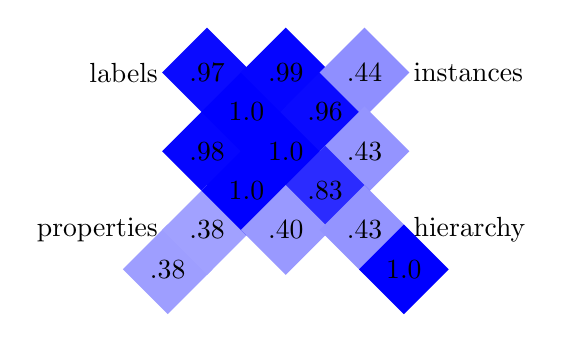
\begin{tikzpicture}
\draw (-.5,2.) node[anchor=east] {labels};
\draw (0,2.) node[diamond,minimum size=.5cm,fill=blue!96] {.97}; % l
\draw (0,1.) node[diamond,minimum size=.5cm,fill=blue!98] {.98}; % lp
\draw (0.5,1.5) node[diamond,minimum size=.5cm,fill=blue!100] {1.0}; % lip
\draw (1.,2.) node[diamond,minimum size=.5cm,fill=blue!98] {.99}; %li

\draw (-.5,0.) node[anchor=east] {properties};
\draw (-0.5,-0.5) node[diamond,minimum size=.5cm,fill=blue!38] {.38}; % ip
\draw (0,0) node[diamond,minimum size=.5cm,fill=blue!37] {.38}; %p
\draw (.5,.5) node[diamond,minimum size=.5cm,fill=blue!100] {1.0}; % lph
\draw (1.,1.) node[diamond,minimum size=.5cm,fill=blue!100] {1.0}; % liph
\draw (1.5,1.5) node[diamond,minimum size=.5cm,fill=blue!96] {.96}; %hil
\draw (2.,2.) node[diamond,minimum size=.5cm,fill=blue!44] {.44}; %i
\draw (2.5,2.0) node[anchor=west] {instances};

\draw (2.,1.) node[diamond,minimum size=.5cm,fill=blue!42] {.43}; % hi
\draw (1.5,0.5) node[diamond,minimum size=.5cm,fill=blue!83] {.83}; % phi
\draw (1.,0) node[diamond,minimum size=.5cm,fill=blue!40] {.40}; % ph
\draw (2.,0) node[diamond,minimum size=.5cm,fill=blue!42] {.43}; % h
\draw (2.5,0.) node[anchor=west] {hierarchy};
\draw (2.5,-0.5) node[diamond,minimum size=.5cm,fill=blue!100] {1.0}; % hl
\end{tikzpicture} 
\caption{SEMA evaluation on F-measure (the darkest the best).}\label{fig:diagSEMA}
\end{center}
\end{floatingfigure}

%% Plot generated by GroupOutput of alignapi
\begin{floatingigure}[r]{6.5cm}
\begin{figure}[!h]
\begin{center}
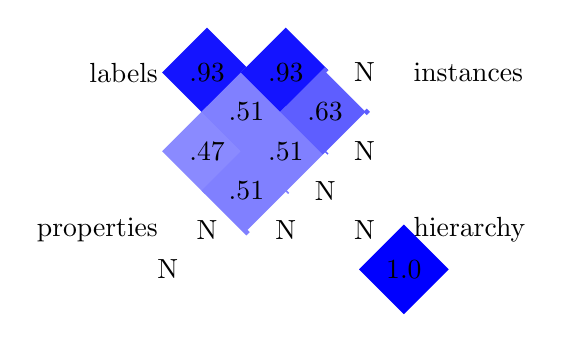
\begin{tikzpicture}
\draw (-.5,2.) node[anchor=east] {labels};
\draw (0,2.) node[diamond,minimum size=.5cm,fill=blue!92] {.93}; % l
\draw (0,1.) node[diamond,minimum size=.5cm,fill=blue!46] {.47}; % lp
\draw (0.5,1.5) node[diamond,minimum size=.5cm,fill=blue!50] {.51}; % lip
\draw (1.,2.) node[diamond,minimum size=.5cm,fill=blue!92] {.93}; %li

\draw (-.5,0.) node[anchor=east] {properties};
\draw (-0.5,-0.5) node[diamond,minimum size=.5cm,fill=blue!0] {N}; % ip
\draw (0,0) node[diamond,minimum size=.5cm,fill=blue!0] {N}; %p
\draw (.5,.5) node[diamond,minimum size=.5cm,fill=blue!50] {.51}; % lph
\draw (1.,1.) node[diamond,minimum size=.5cm,fill=blue!50] {.51}; % liph
\draw (1.5,1.5) node[diamond,minimum size=.5cm,fill=blue!63] {.63}; %hil
\draw (2.,2.) node[diamond,minimum size=.5cm,fill=blue!0] {N}; %i
\draw (2.5,2.0) node[anchor=west] {instances};

\draw (2.,1.) node[diamond,minimum size=.5cm,fill=blue!0] {N}; % hi
\draw (1.5,0.5) node[diamond,minimum size=.5cm,fill=blue!0] {N}; % phi
\draw (1.,0) node[diamond,minimum size=.5cm,fill=blue!0] {N}; % ph
\draw (2.,0) node[diamond,minimum size=.5cm,fill=blue!0] {N}; % h
\draw (2.5,0.) node[anchor=west] {hierarchy};
\draw (2.5,-0.5) node[diamond,minimum size=.5cm,fill=blue!100] {1.0}; % hl
\end{tikzpicture} 
\caption{TaxoMap evaluation on F-measure (the darkest the best).}\label{fig:diagTaxoMap}
\end{center}
\end{floatingfigure}

%% Plot generated by GroupOutput of alignapi
\begin{floatingigure}[r]{6.5cm}
\begin{figure}[!h]
\begin{center}
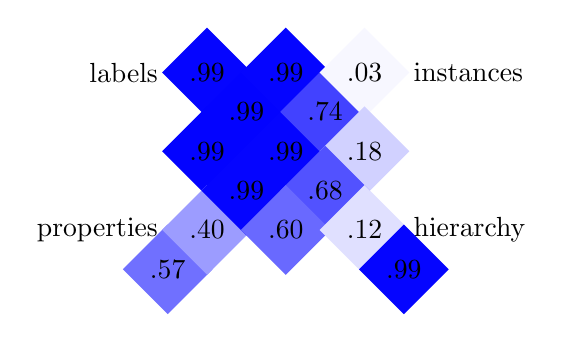
\begin{tikzpicture}
\draw (-.5,2.) node[anchor=east] {labels};
\draw (0,2.) node[diamond,minimum size=.5cm,fill=blue!98] {.99}; % l
\draw (0,1.) node[diamond,minimum size=.5cm,fill=blue!99] {.99}; % lp
\draw (0.5,1.5) node[diamond,minimum size=.5cm,fill=blue!99] {.99}; % lip
\draw (1.,2.) node[diamond,minimum size=.5cm,fill=blue!98] {.99}; %li

\draw (-.5,0.) node[anchor=east] {properties};
\draw (-0.5,-0.5) node[diamond,minimum size=.5cm,fill=blue!56] {.57}; % ip
\draw (0,0) node[diamond,minimum size=.5cm,fill=blue!39] {.40}; %p
\draw (.5,.5) node[diamond,minimum size=.5cm,fill=blue!98] {.99}; % lph
\draw (1.,1.) node[diamond,minimum size=.5cm,fill=blue!98] {.99}; % liph
\draw (1.5,1.5) node[diamond,minimum size=.5cm,fill=blue!74] {.74}; %hil
\draw (2.,2.) node[diamond,minimum size=.5cm,fill=blue!3] {.03}; %i
\draw (2.5,2.0) node[anchor=west] {instances};

\draw (2.,1.) node[diamond,minimum size=.5cm,fill=blue!18] {.18}; % hi
\draw (1.5,0.5) node[diamond,minimum size=.5cm,fill=blue!68] {.68}; % phi
\draw (1.,0) node[diamond,minimum size=.5cm,fill=blue!59] {.60}; % ph
\draw (2.,0) node[diamond,minimum size=.5cm,fill=blue!12] {.12}; % h
\draw (2.5,0.) node[anchor=west] {hierarchy};
\draw (2.5,-0.5) node[diamond,minimum size=.5cm,fill=blue!98] {.99}; % hl
\end{tikzpicture} 
\caption{xsom evaluation on F-measure (the darkest the best).}\label{fig:diagxsom}
\end{center}
\end{floatingfigure}
\end{document}

